\documentclass[10pt]{beamer}

\usetheme{default} % theme général du diaporama

% paquets pour le français
\usepackage[T1]{fontenc}
\usepackage[utf8]{inputenc}
\usepackage{graphicx}

\title{Identification spatiale continue des points chauds de diversité beta à l'aide de modèles de distribution d'espèces}
\author{Gabriel Dansereau}

\begin{document}

\begin{frame}
  \titlepage
\end{frame}

\begin{frame}
  \frametitle{Plan de la présentation}
  \begin{itemize}
    \item Objectif
    \item Description eBird
    \item Données BIOCLIM
    \item Données brutes
    \begin{itemize}
      \item Méthode présence-absence
      \item Résultats
    \end{itemize}
    \item Modèles de distribution d'espèces (SDM)
    \begin{itemize}
      \item Méthode BIOCLIM
      \item Résultats
    \end{itemize}
    \item À venir
    \item Autres points
  \end{itemize}
\end{frame}

\begin{frame}
  \frametitle{Objectif}
  \begin{itemize}
    \item Objectif général: Identification des zones qui contribuent le plus à la diversité beta dans l'espace
    \begin{itemize}
      \item Échelle continue, étendue
      \item Diversité beta: composition spécifique, interactions
      \item Prévision changements climatiques
      \item Données science ouverte \& science citoyenne
    \end{itemize}
    \medskip
    \item 1ère partie: Test de la méthode
    \begin{itemize}
      \item LCBD sur données brutes
      \item Développement méthode SDM
      \item LCBD sur sorties SDM
      \item Scénarios changements climatiques IPCC
    \end{itemize}
    \medskip
    \item 2e partie: Applications aux interactions
  \end{itemize}
\end{frame}

\begin{frame}
  \frametitle{Description eBird}
  \begin{itemize}
    \item Parulines - Famille Parulidae
    \item CA, US, MX
    \item 23 000 000 observations (uniques)
    \item 63 espèces: quartiles = 2, 11 000, 140 000, 370 000, 4 000 000
    \item Années: quartiles = 1838, 2012, 2015, 2018, 2019
  \end{itemize}
\end{frame}

\begin{frame}
  \frametitle{Description eBird}
  \begin{itemize}
    \item Variables base : espèce, latitude, longitude, date, checklist complète, compte
  \end{itemize}
  \resizebox{\textwidth}{!}{%
  \begin{table}[ht]
    \centering
    \begin{tabular}{rlrrlrl}
      \small
      \hline
      & species & latitude & longitude & observationDate & allSpeciesReported &   observationCount \\
      \hline
      1 & Setophaga\_townsendi & 35.32 & -120.84 & 2007-03-17 &   1 & 1 \\
      2 & Geothlypis\_trichas & 35.32 & -120.84 & 1994-11-06 &   1 & 4 \\
      3 & Oreothlypis\_celata & 58.35 & -134.59 & 2008-07-22 &   1 & 2 \\
      4 & Setophaga\_coronata & 58.35 & -134.59 & 2008-07-22 &   1 & 1 \\
      5 & Setophaga\_coronata & 49.10 & -123.17 & 1979-10-16 &   1 & 8 \\
      6 & Setophaga\_coronata & 37.90 & -75.37 & 2004-11-23 &   1 & 82 \\
      \hline
    \end{tabular}
  \end{table}
  }
  \begin{itemize}
    \item Données échantillonnage: type échantillonnage, durée, distance, nombre d'observateurs
  \end{itemize}
  \resizebox{\textwidth}{!}{%
    \begin{table}[ht]
      \centering
      \begin{tabular}{rlrrr}
        \small
        \hline
        & protocolType & durationMinutes & effortDistanceKm & numberObservers \\
        \hline
        1 & Area &  60 &  &  15 \\
        2 & Historical &  30 &  &   1 \\
        3 & Traveling &  50 & 2.09 &   1 \\
        4 & Traveling &  50 & 2.09 &   1 \\
        5 & Incidental &  &  &   1 \\
        6 & Traveling & 105 & 2.58 &   5 \\
        \hline
      \end{tabular}
    \end{table}
  }
\end{frame}

\begin{frame}
  \frametitle{SDM - Données BIOCLIM}
  \resizebox{\textwidth}{!}{%
    \begin{table}
      \begin{tabular}{l|l}
        \small
        \hline
        Variable & Description                                                \\
        \hline
        1        & Annual Mean Temperature                                    \\
        2        & Mean Diurnal Range (Mean of monthly (max temp - min temp)) \\
        3        & Isothermality (BIO2/BIO7) (* 100)                          \\
        4        & Temperature Seasonality (standard deviation *100)          \\
        5        & Max Temperature of Warmest Month                           \\
        6        & Min Temperature of Coldest Month                           \\
        7        & Temperature Annual Range (BIO5-BIO6)                       \\
        8        & Mean Temperature of Wettest Quarter                        \\
        9        & Mean Temperature of Driest Quarter                         \\
        10       & Mean Temperature of Warmest Quarter                        \\
        11       & Mean Temperature of Coldest Quarter                        \\
        12       & Annual Precipitation                                       \\
        13       & Precipitation of Wettest Month                             \\
        14       & Precipitation of Driest Month                              \\
        15       & Precipitation Seasonality (Coefficient of Variation)       \\
        16       & Precipitation of Wettest Quarter                           \\
        17       & Precipitation of Driest Quarter                            \\
        18       & Precipitation of Warmest Quarter                           \\
        19       & Precipitation of Coldest Quarter                           \\
        \hline
      \end{tabular}
    \end{table}
  }
\end{frame}

\begin{frame}
  \vfill
  \centering
  \huge Données brutes
  \vfill
\end{frame}

\begin{frame}
  \frametitle{Données brutes - Méthodes}
  Presence-absence par espèce
  \begin{itemize}
    \item Pixels - Résolution 5 arc-minutes
    \item Matrice 661 x 1141 (env. 750 000 pixels)
    \item 100 000 sites avec observations sur 400 000 sites
  \end{itemize}
  \medskip
  Matrice Y sites x espèces
  \begin{itemize}
    \item 100 000 x 63
    \item Transformation Hellinger
  \end{itemize}
  \medskip
  Calcul LCBD
  \begin{itemize}
    \item Var(Y), SStotal, BDtotal, SSi, LCBDi...
    \item Test permutation (correction?)
  \end{itemize}
\end{frame}

\begin{frame}
  \frametitle{Données brutes - 1 espèce, beaucoup d'observations}
  \begin{figure}
    \centering
    \hspace*{-2cm}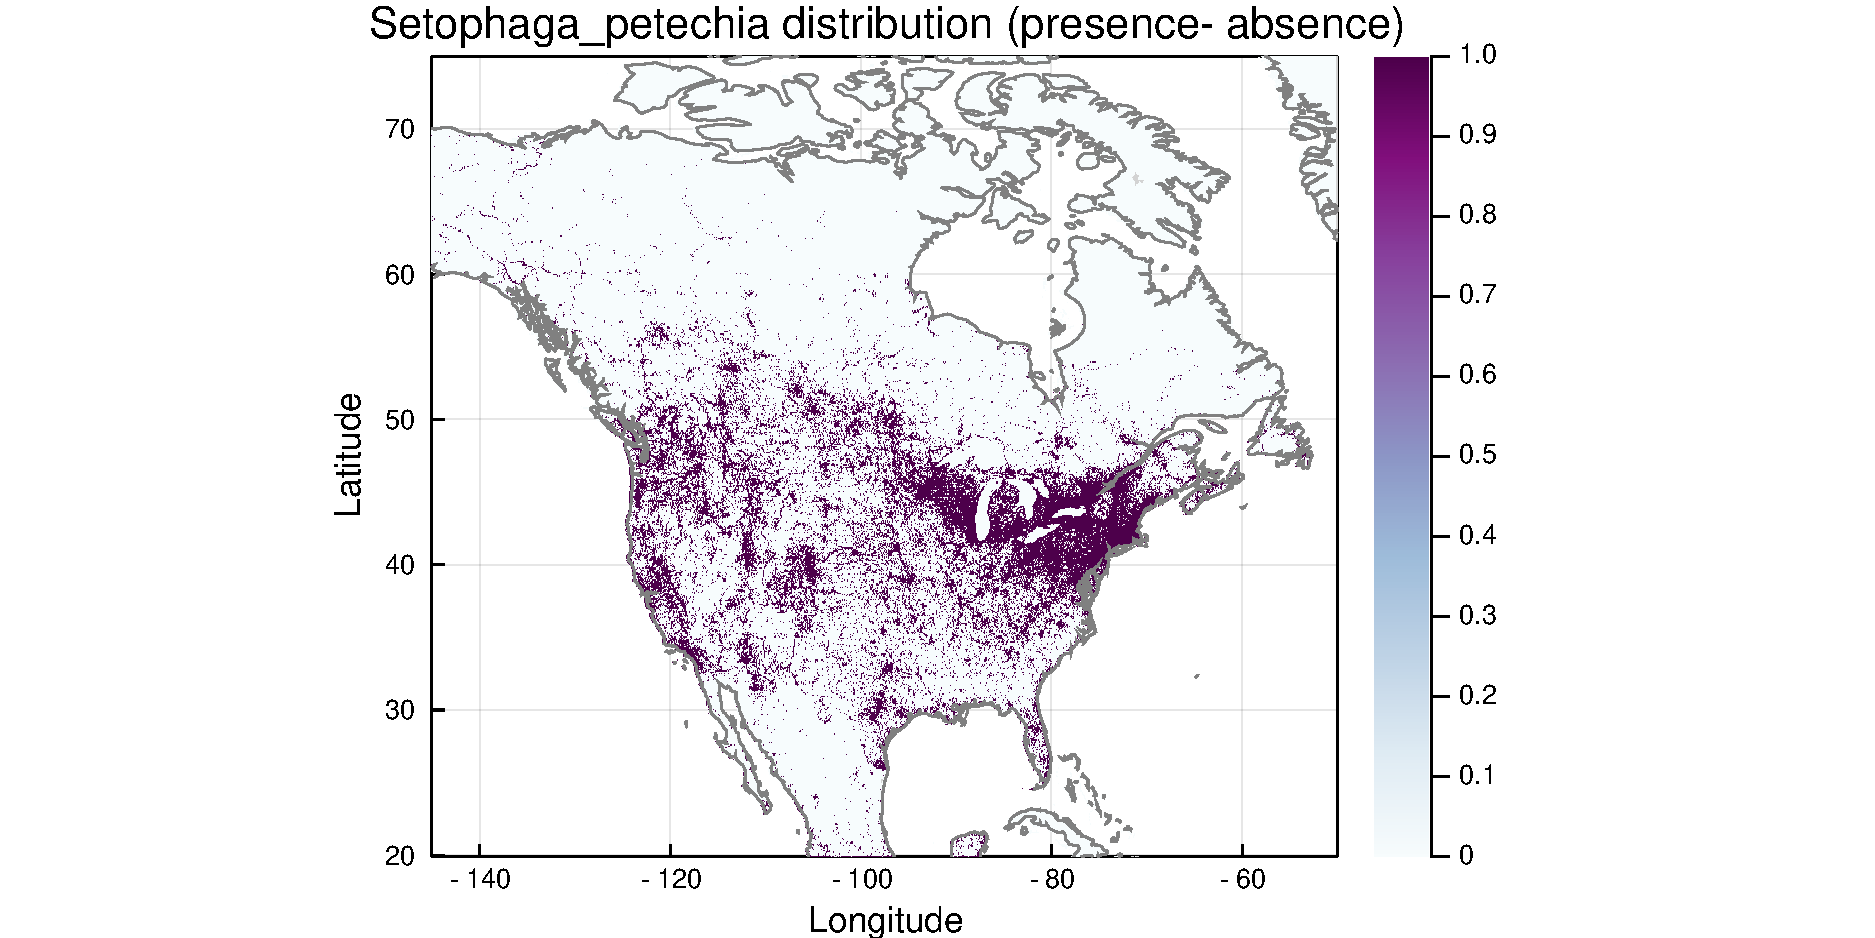
\includegraphics[scale=0.5]{../fig/raw/raw-sp-Setophaga_petechia.pdf}
    \caption{Distribution des observations de la Paruline jaune (présence-absence)}
  \end{figure}
\end{frame}

\begin{frame}
  \frametitle{Données brutes - 1 espèce, moins d'observations}
  \begin{figure}
    \centering
    \hspace*{-2cm}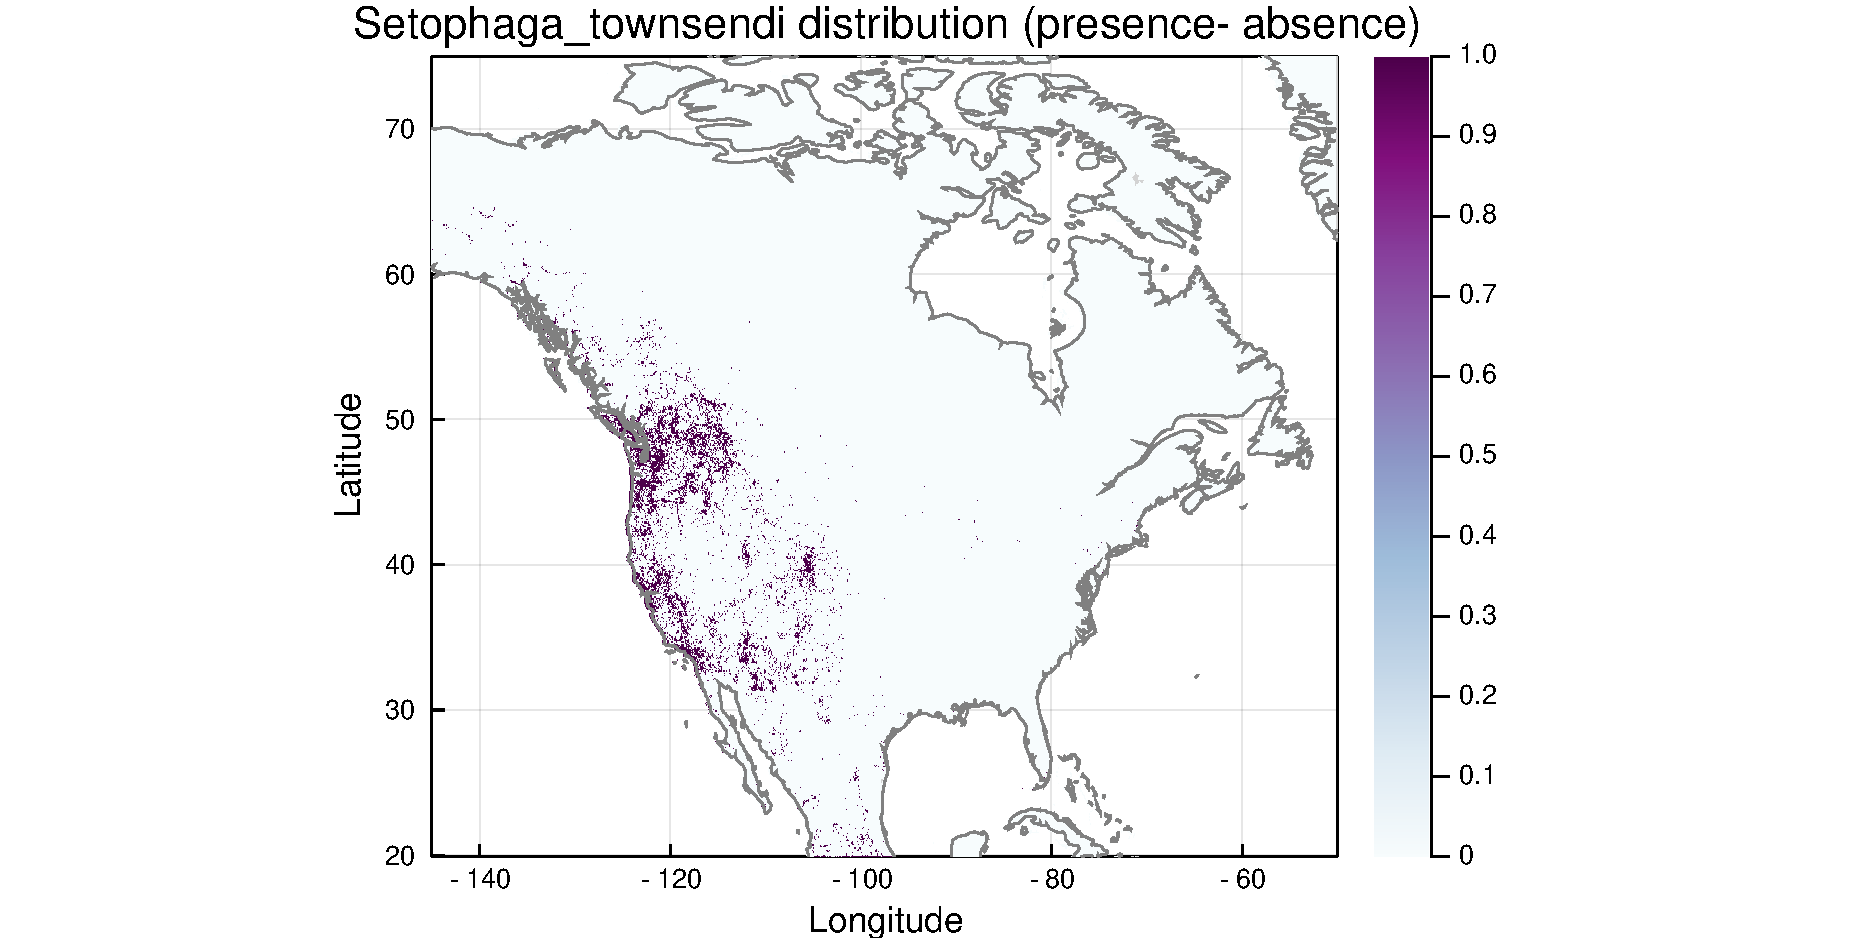
\includegraphics[scale=0.5]{../fig/raw/raw-sp-Setophaga_townsendi.pdf}
    \caption{Distribution des observations de la Paruline de Townsend (présence-absence)}
  \end{figure}
\end{frame}

\begin{frame}
  \frametitle{Données brutes - Matrice Y (non triée)}
  \begin{figure}
    \centering
    \hspace*{-2cm}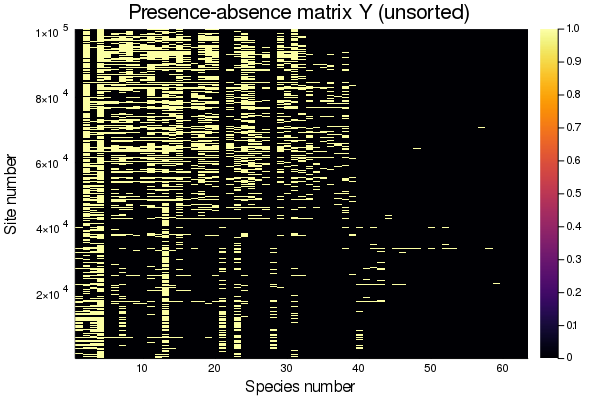
\includegraphics[scale=0.5]{../fig/raw/raw-Y-unsorted.png}
  \end{figure}
\end{frame}

\begin{frame}
  \frametitle{Données brutes - Matrice Y (triée par richesse, puis fréquence)}
  \begin{figure}
    \centering
    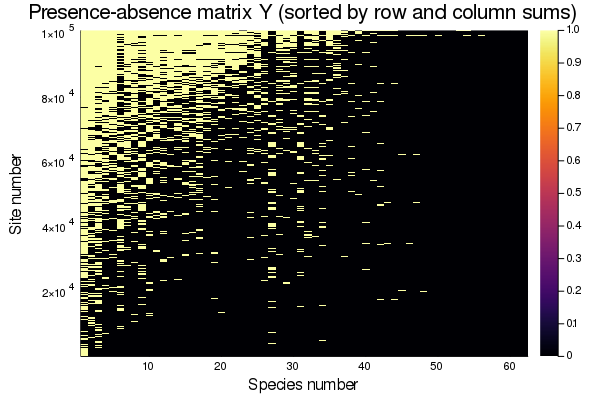
\includegraphics[scale=0.4]{../fig/raw/raw-Y-rowcolsorted.png}
  \end{figure}
\end{frame}

\begin{frame}
  \frametitle{Données brutes - Richesse spécifique (nombre d'espèces)}
  \begin{figure}
    \centering
    \hspace*{-2cm}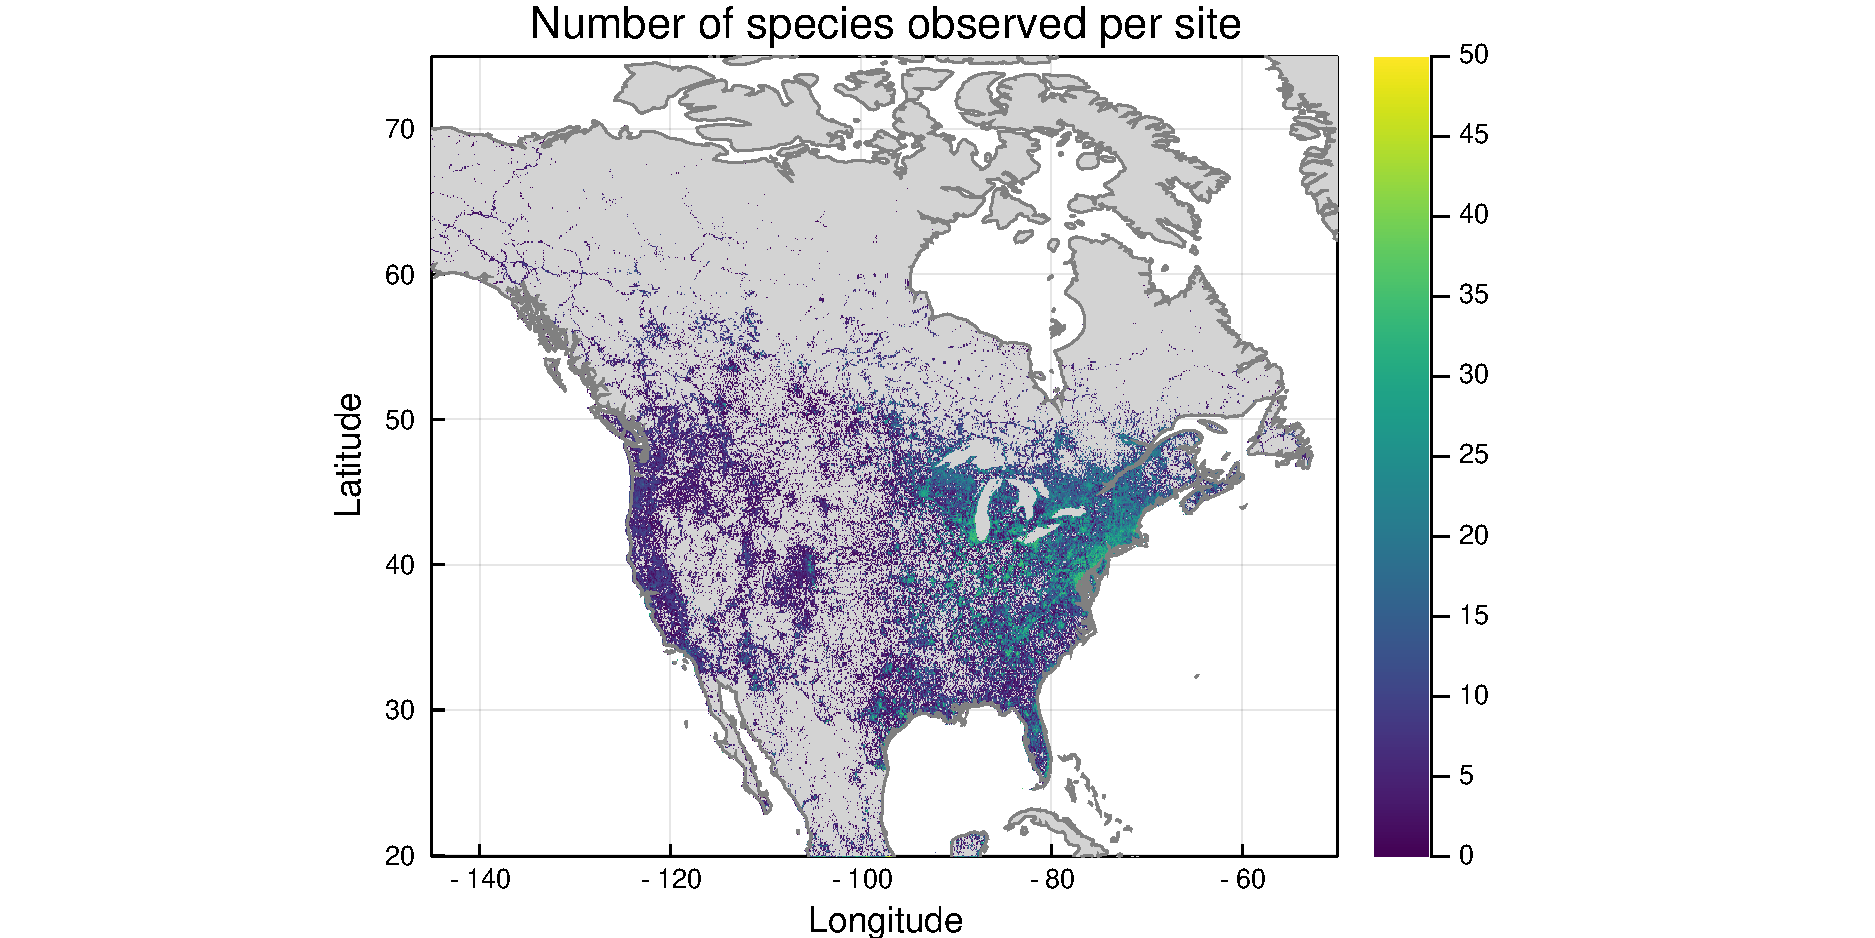
\includegraphics[scale=0.5]{../fig/raw/raw-richness.pdf}
  \end{figure}
\end{frame}

\begin{frame}
  \frametitle{Données brutes - Diversité spécifique}
  \begin{figure}
    \centering
    \hspace*{-2cm}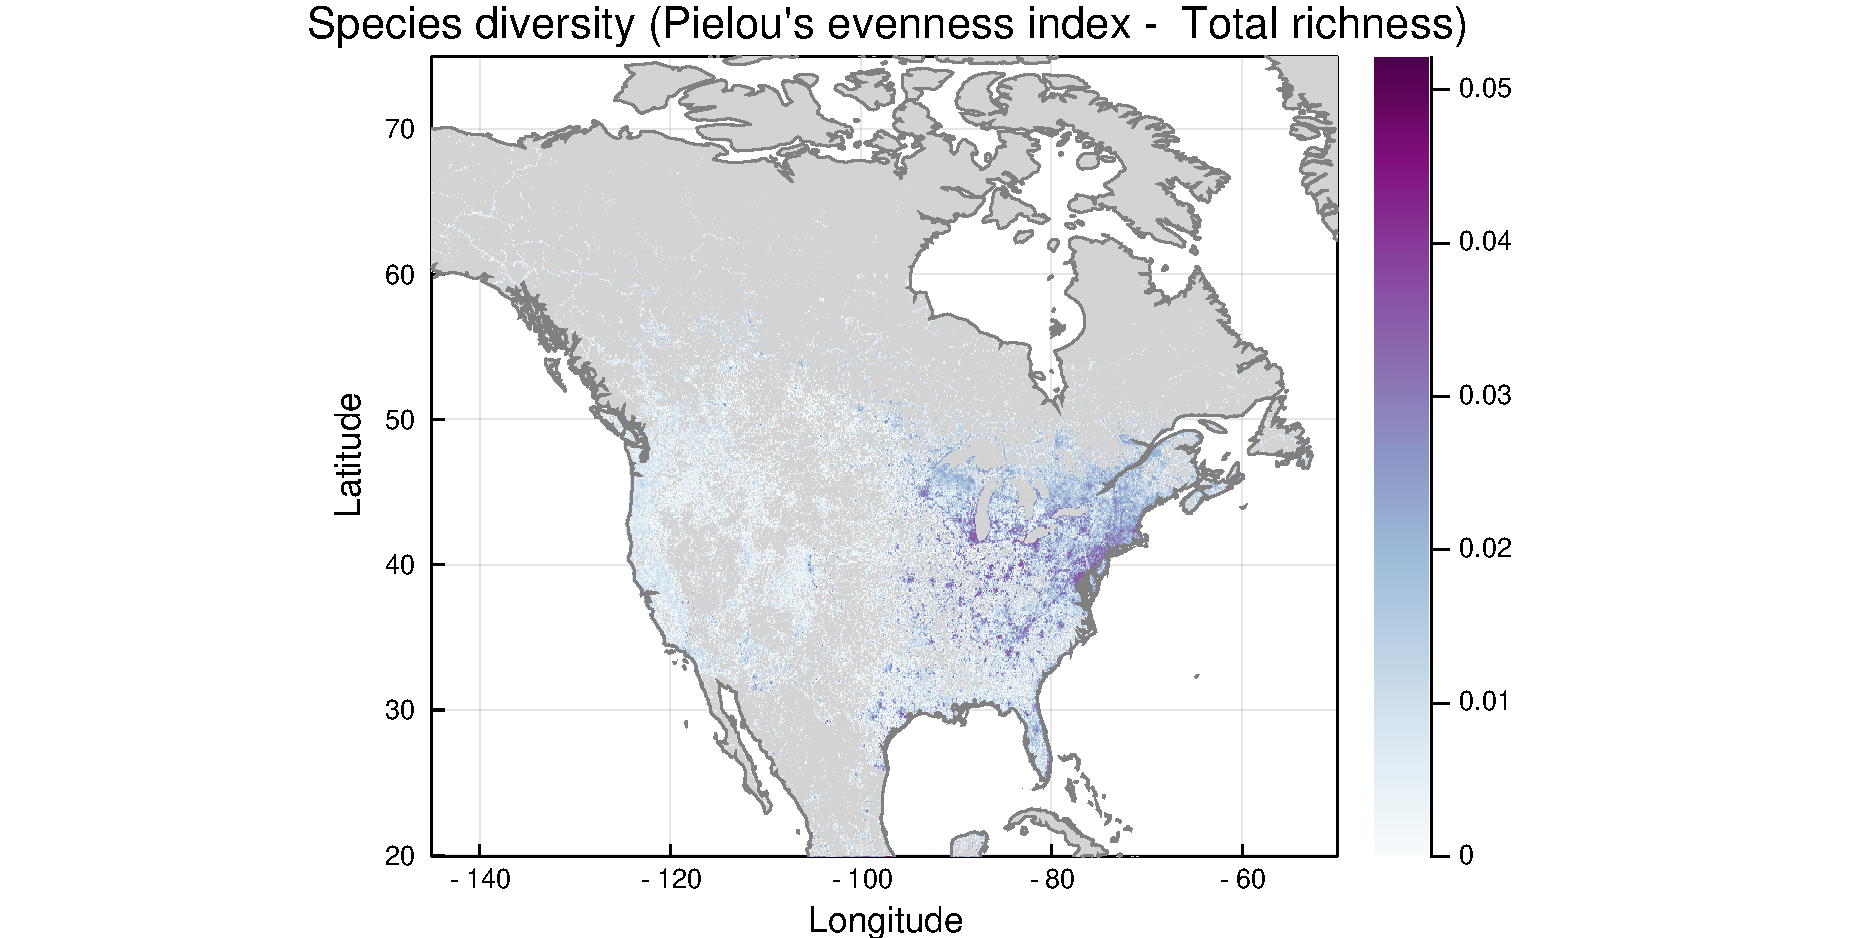
\includegraphics[scale=0.5]{../fig/raw/raw-diversity-pielou2.pdf}
  \end{figure}
\end{frame}

\begin{frame}
  \frametitle{Données brutes - Diversité spécifique}
  \begin{figure}
    \centering
    \hspace*{-2cm}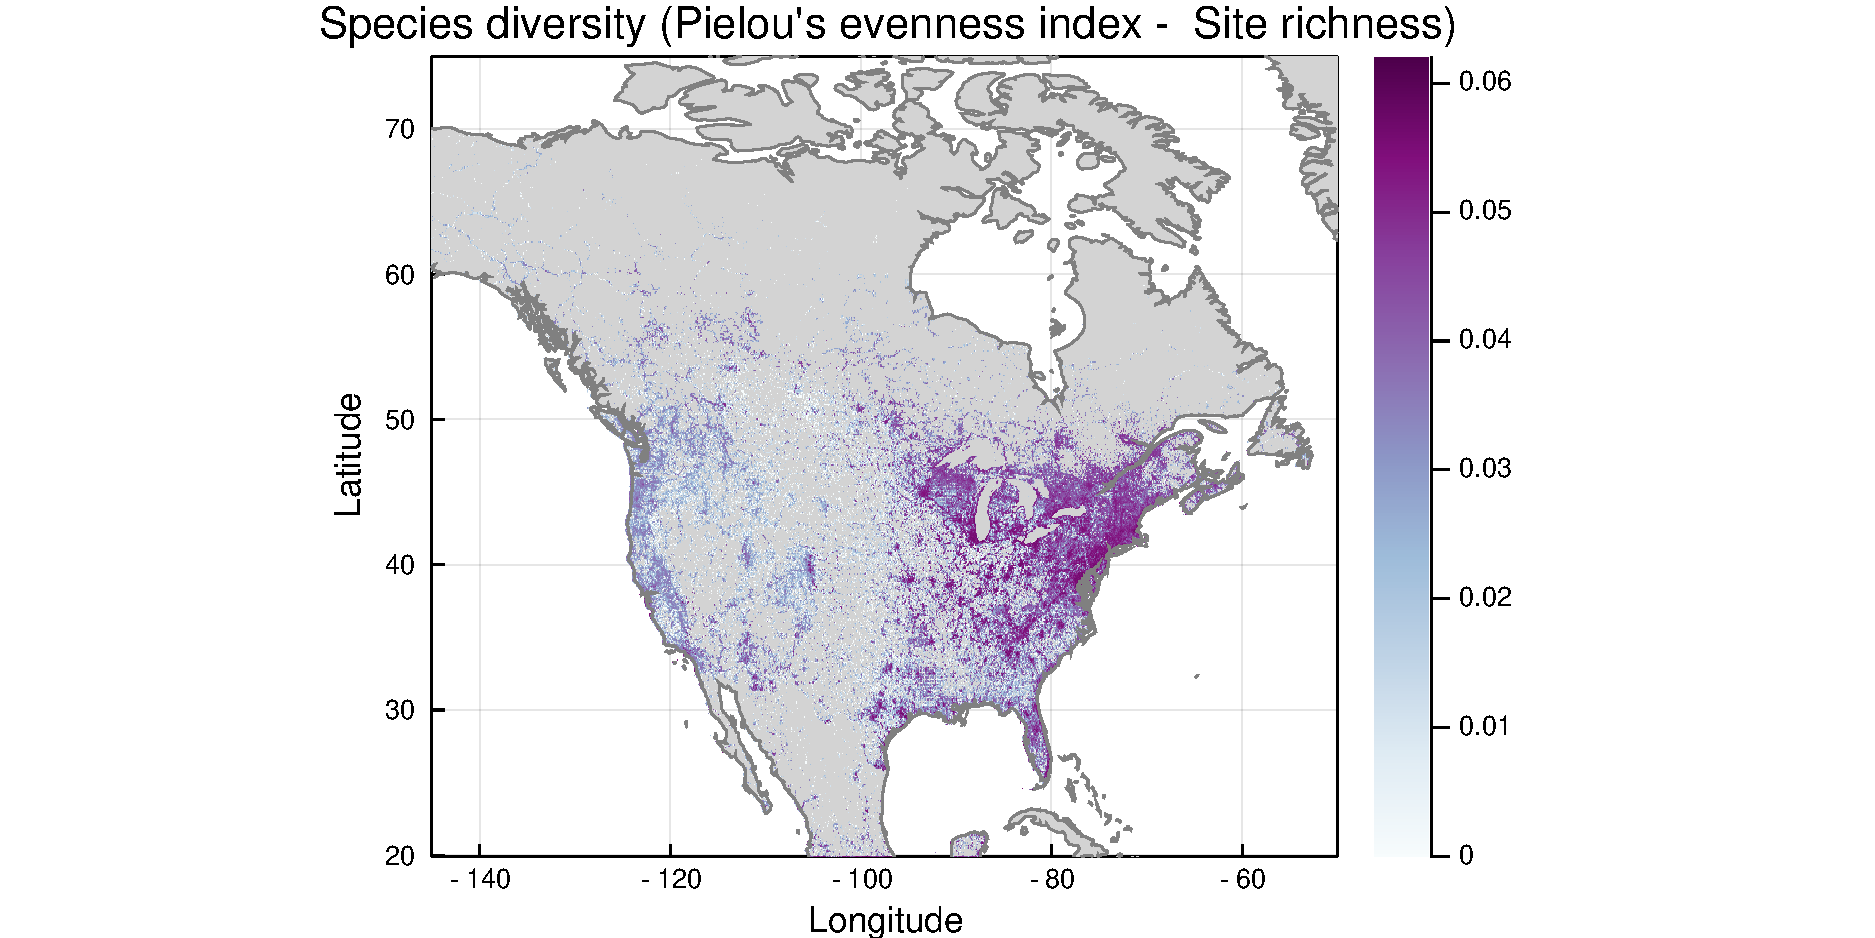
\includegraphics[scale=0.5]{../fig/raw/raw-diversity-pielou.pdf}
  \end{figure}
\end{frame}

\begin{frame}
  \frametitle{Données brutes- LCBD}
  \begin{figure}
    \centering
    \hspace*{-2cm}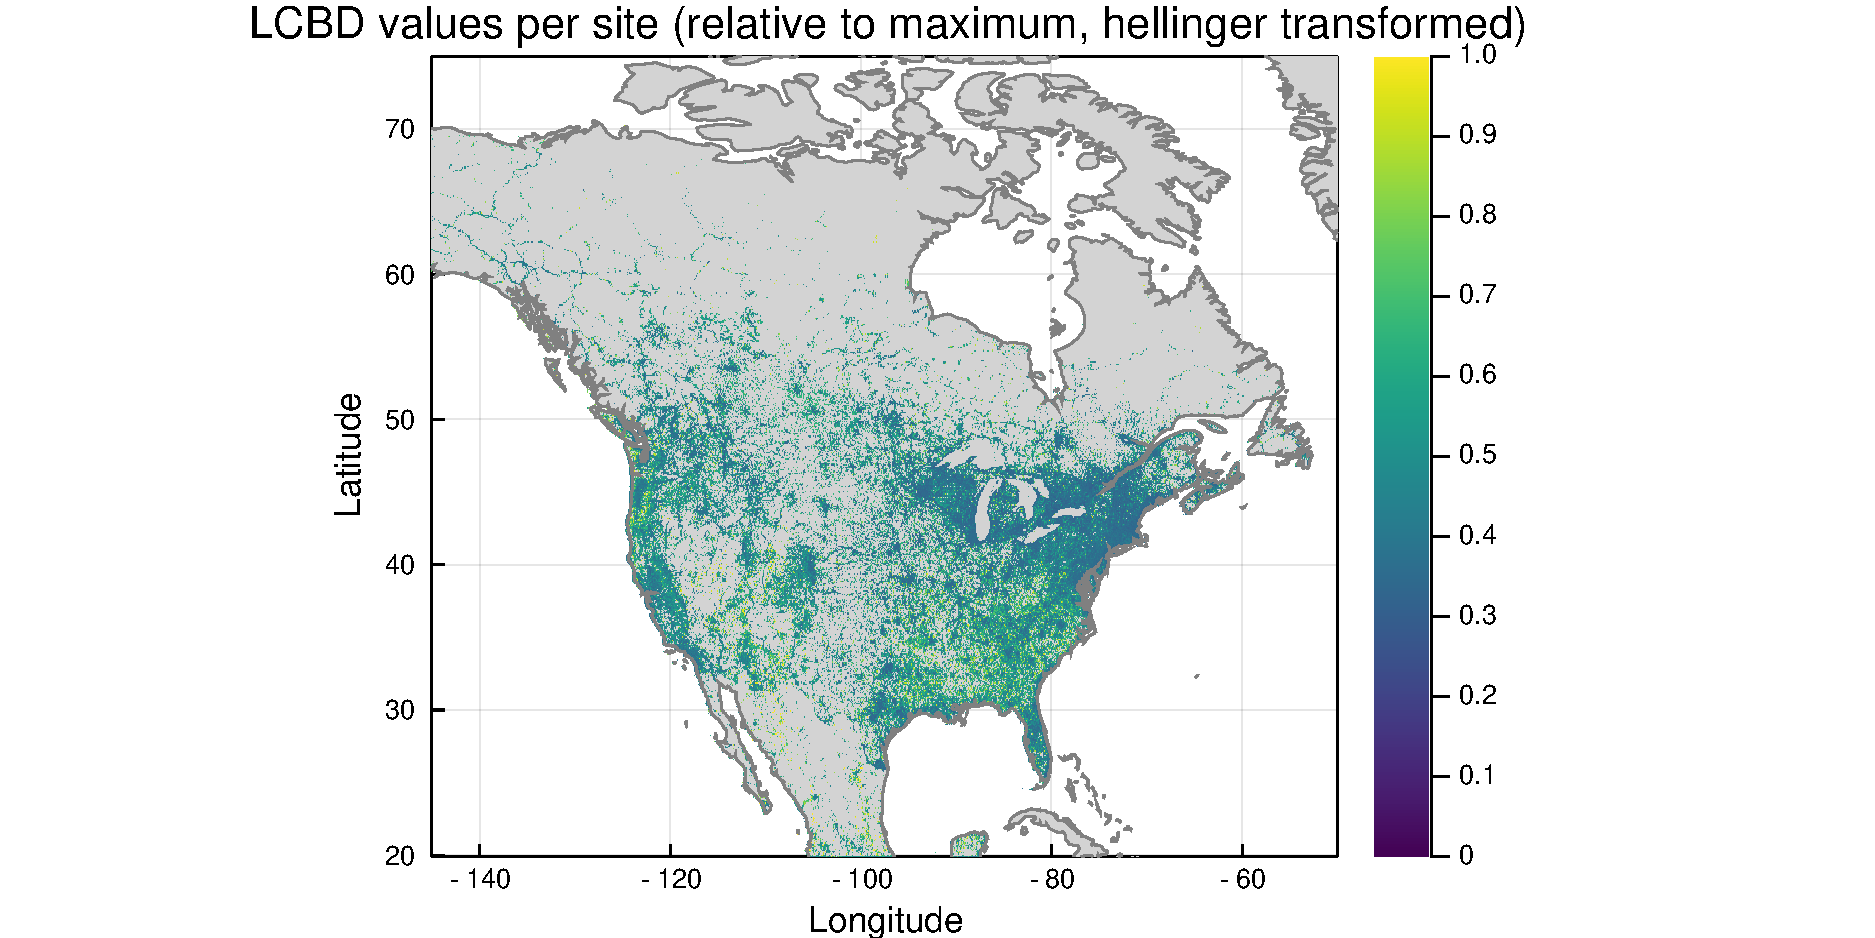
\includegraphics[scale=0.5]{../fig/raw/raw-lcbd-transf.pdf}
  \end{figure}
\end{frame}

\begin{frame}
  \frametitle{Données brutes - LCBD significatives}
  \begin{figure}
    \centering
    \hspace*{-2cm}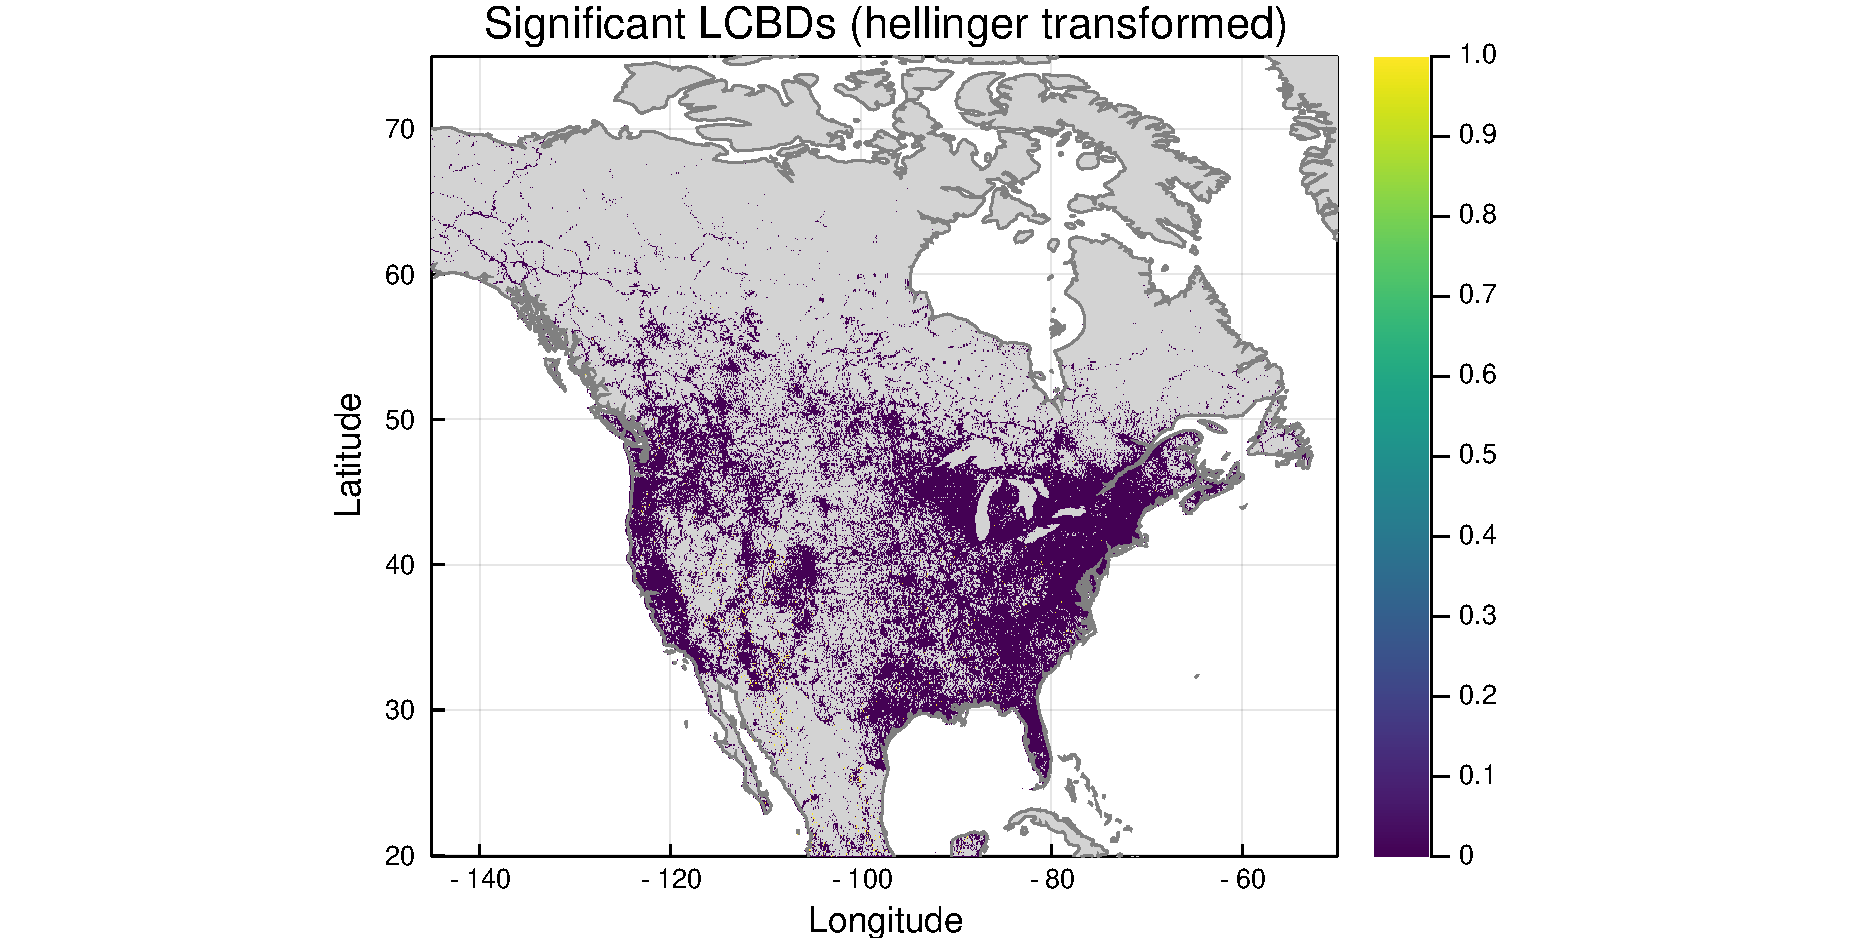
\includegraphics[scale=0.5]{../fig/raw/raw-lcbd-signif.pdf}
  \end{figure}
\end{frame}

\begin{frame}
  \frametitle{Données brutes - Relation LCBD-richesse}
  \begin{figure}
    \centering
    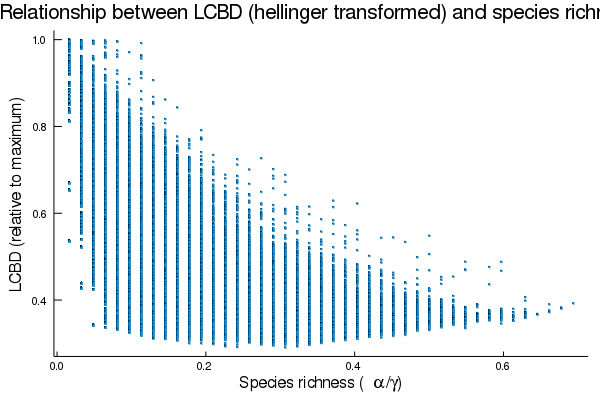
\includegraphics[scale=0.4]{../fig/raw/raw-relation-lcbd-richness-transf.png}
  \end{figure}
\end{frame}


%%%%%%%%%%%%%%%%%%%%%%%%%%%%%%%%%%%%%%

\begin{frame}
  \vfill
  \centering
  \huge SDM
  \vfill
\end{frame}

\begin{frame}
  \frametitle{SDM - Méthode BIOCLIM}
  \begin{figure}
    \centering
    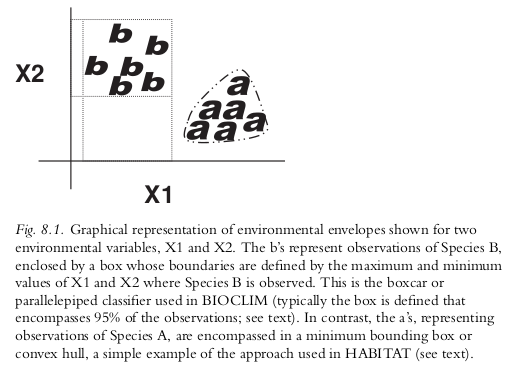
\includegraphics[scale=0.4]{bioclim-with-caption.png}
    \caption{BIOCLIM representation (from Franklin 2010)}
  \end{figure}
\end{frame}

\begin{frame}
  \frametitle{SDM - Méthode BIOCLIM}
  \begin{itemize}
    \item Méthode « climate-envelope-model » classique (Nix 1986)
    \item Boxcar/parallelepiped/hyper-box
    \item Valeur env min-max pour 95\% observations
  \end{itemize}
  Fonctionnement
  \begin{itemize}
    \item Distribution percentile var.env des sites connus
    \item Comparaison chaque variable site inconnu, score 0 à 1
    \item Loi Liebig du minimum, prédiction = variable avec plus petit score
  \end{itemize}
  Avantages
  \begin{itemize}
    \item Simplicité conceptuelle
    \item Utilisation très répandue
  \end{itemize}
  \begin{figure}
    \centering
    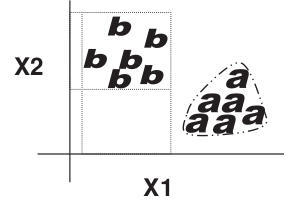
\includegraphics[scale=0.4]{bioclim-fig-only.png}
  \end{figure}
\end{frame}

\begin{frame}
  \frametitle{SDM - 1 espèce, beaucoup d'observations}
  \begin{figure}
    \centering
    \hspace*{-2cm}\includegraphics[scale=0.5]{../fig/sdm/sdm-sp-Setophaga_petechia.pdf}
    \caption{Sortie du SDM pour la Paruline jaune}
  \end{figure}
\end{frame}

\begin{frame}
  \frametitle{SDM - 1 espèce, moins d'observations}
  \begin{figure}
    \centering
    \hspace*{-2cm}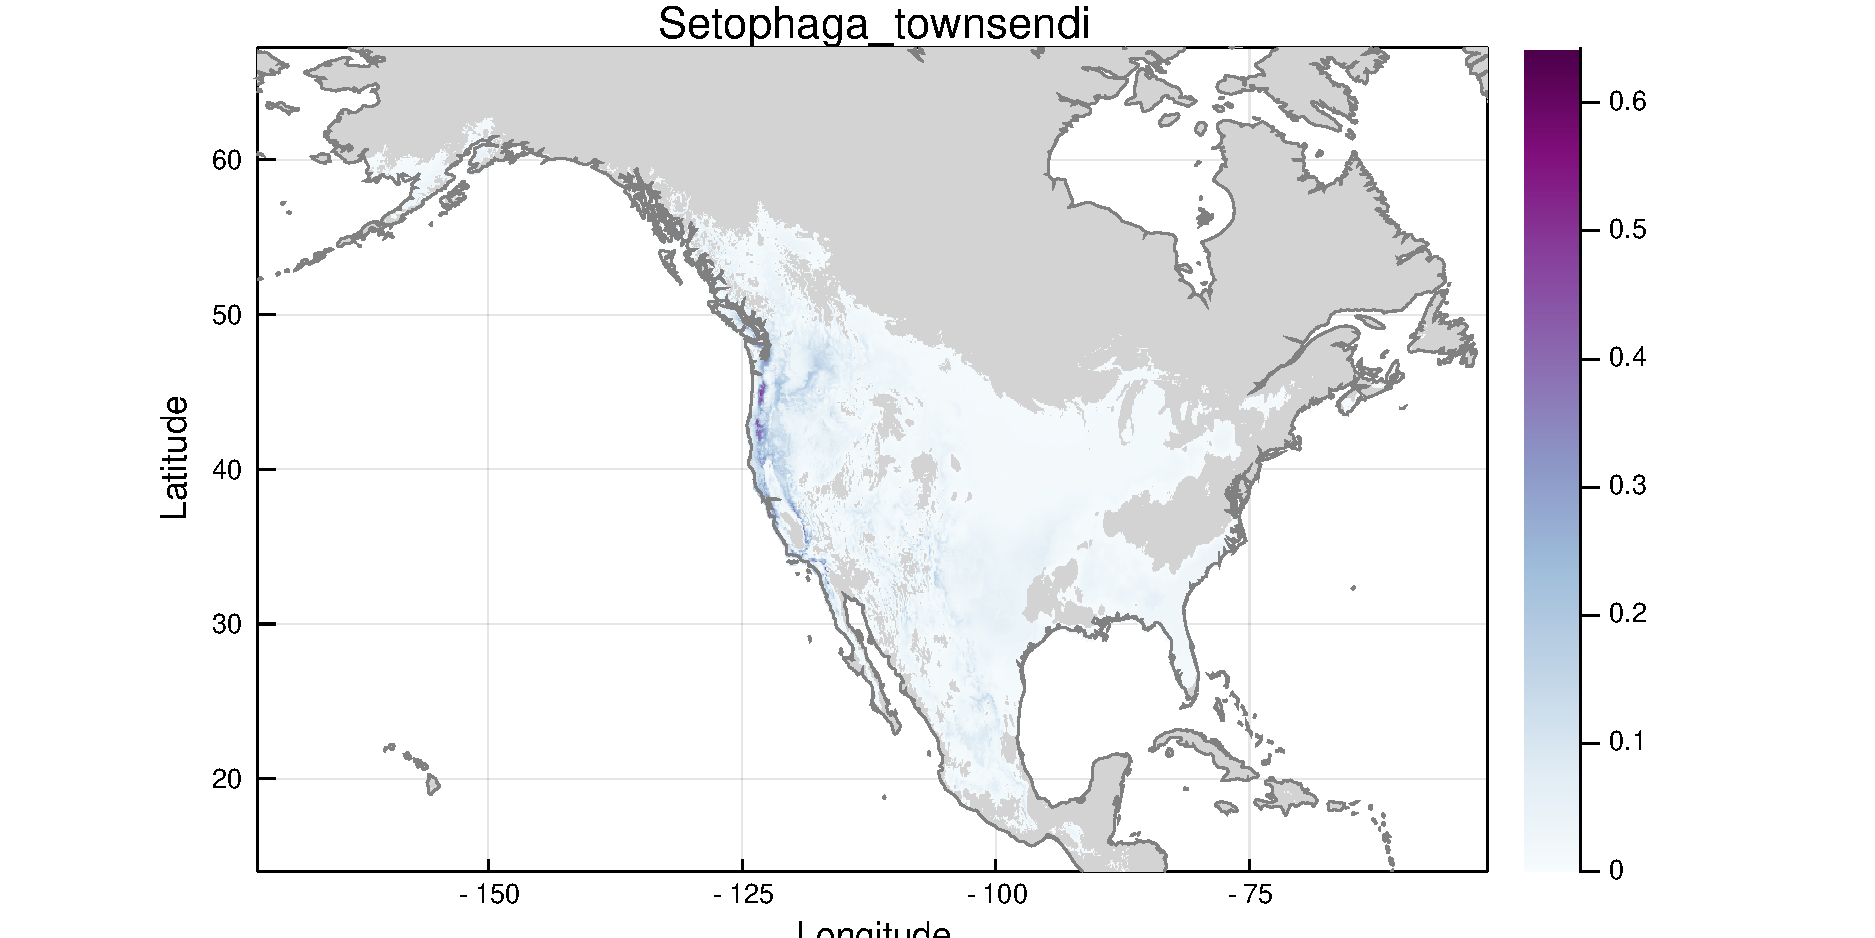
\includegraphics[scale=0.5]{../fig/sdm/sdm-sp-Setophaga_townsendi.pdf}
    \caption{Sortie du SDM pour la Paruline de Townsend}
  \end{figure}
\end{frame}

\begin{frame}
  \frametitle{SDM - Matrice Y (non triée)}
  \begin{figure}
    \centering
    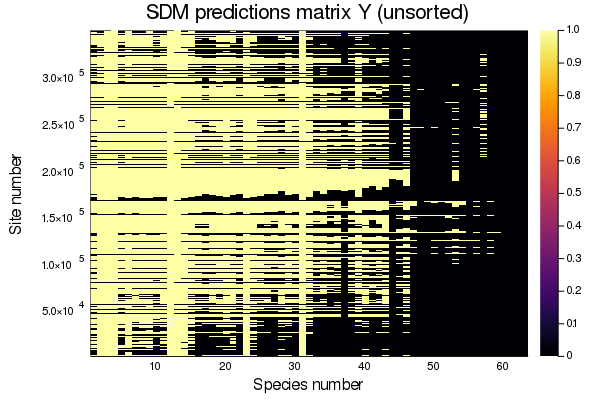
\includegraphics[scale=0.4]{../fig/sdm/sdm-Y-unsorted.png}
  \end{figure}
\end{frame}

\begin{frame}
  \frametitle{SDM - Matrice Y (triée par richesse, puis fréquence)}
  \begin{figure}
    \centering
    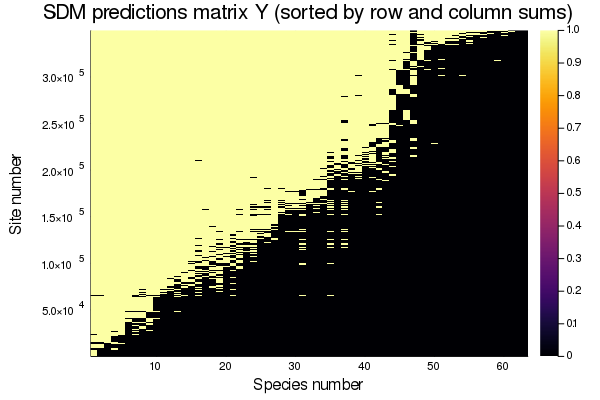
\includegraphics[scale=0.4]{../fig/sdm/sdm-Y-rowcolsorted.png}
  \end{figure}
\end{frame}

\begin{frame}
  \frametitle{SDM- Richesse spécifique (nombre d'espèces)}
  \begin{figure}
    \centering
    \hspace*{-2cm}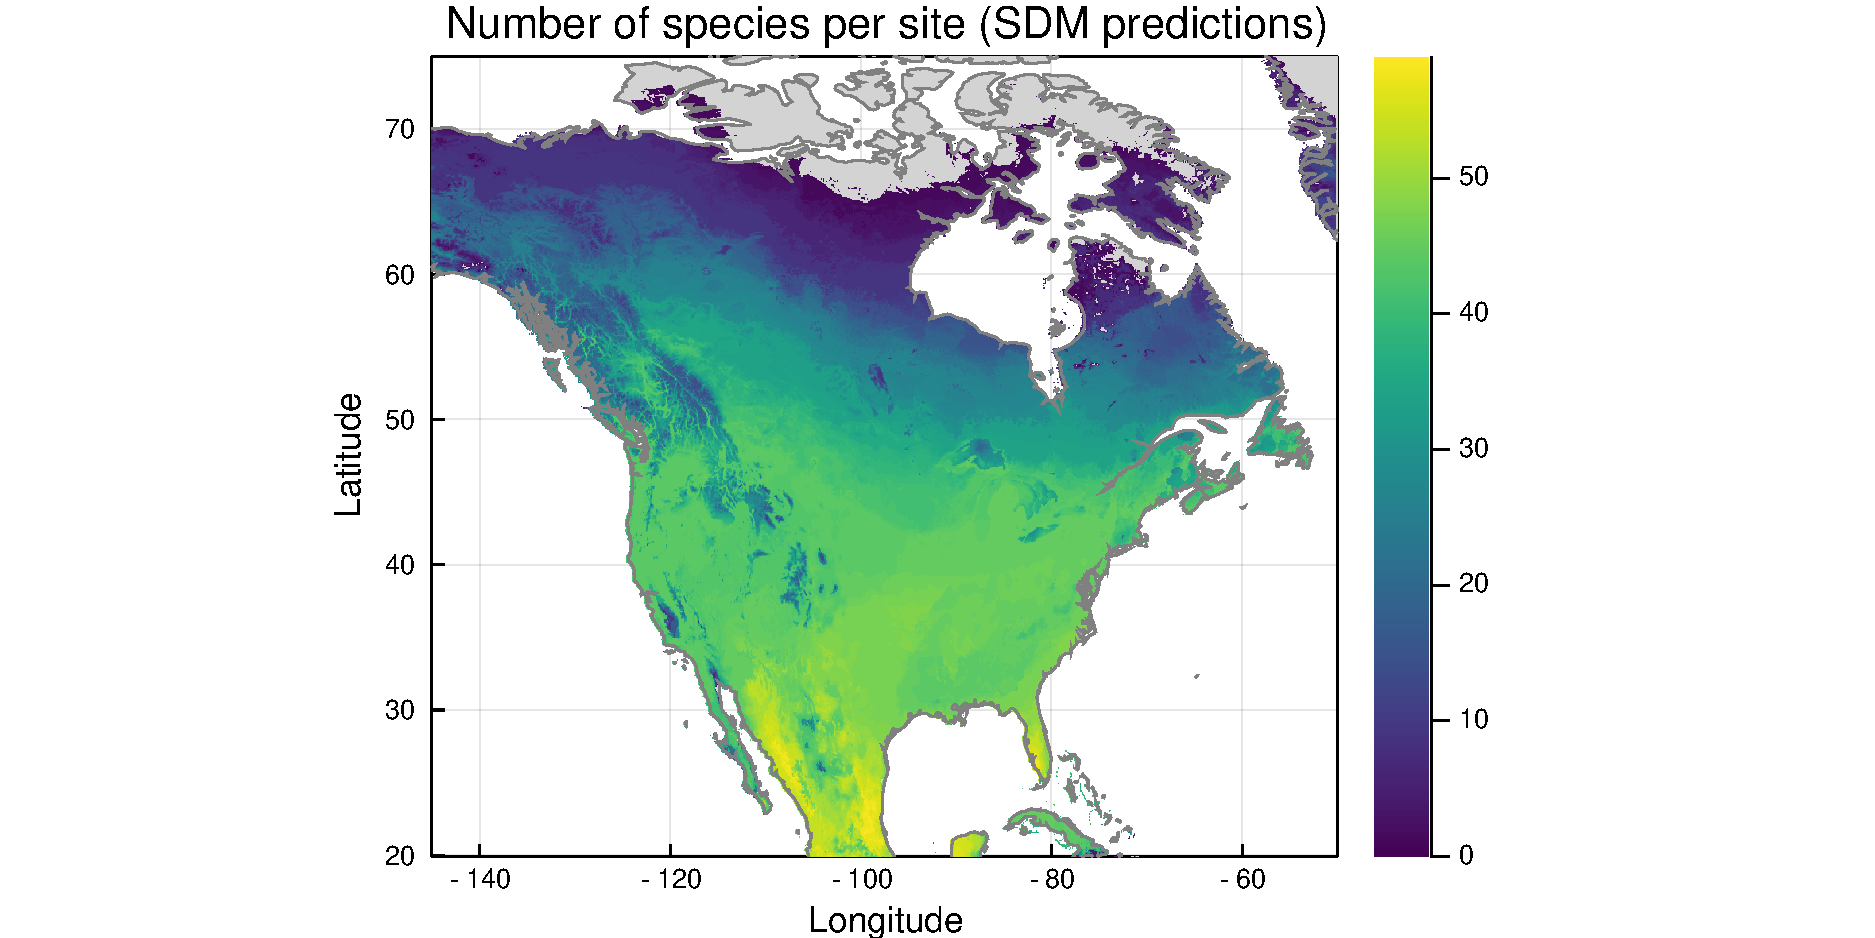
\includegraphics[scale=0.5]{../fig/sdm/sdm-richness.pdf}
  \end{figure}
\end{frame}

\begin{frame}
  \frametitle{SDM - Diversité spécifique}
  \begin{figure}
    \centering
    \hspace*{-2cm}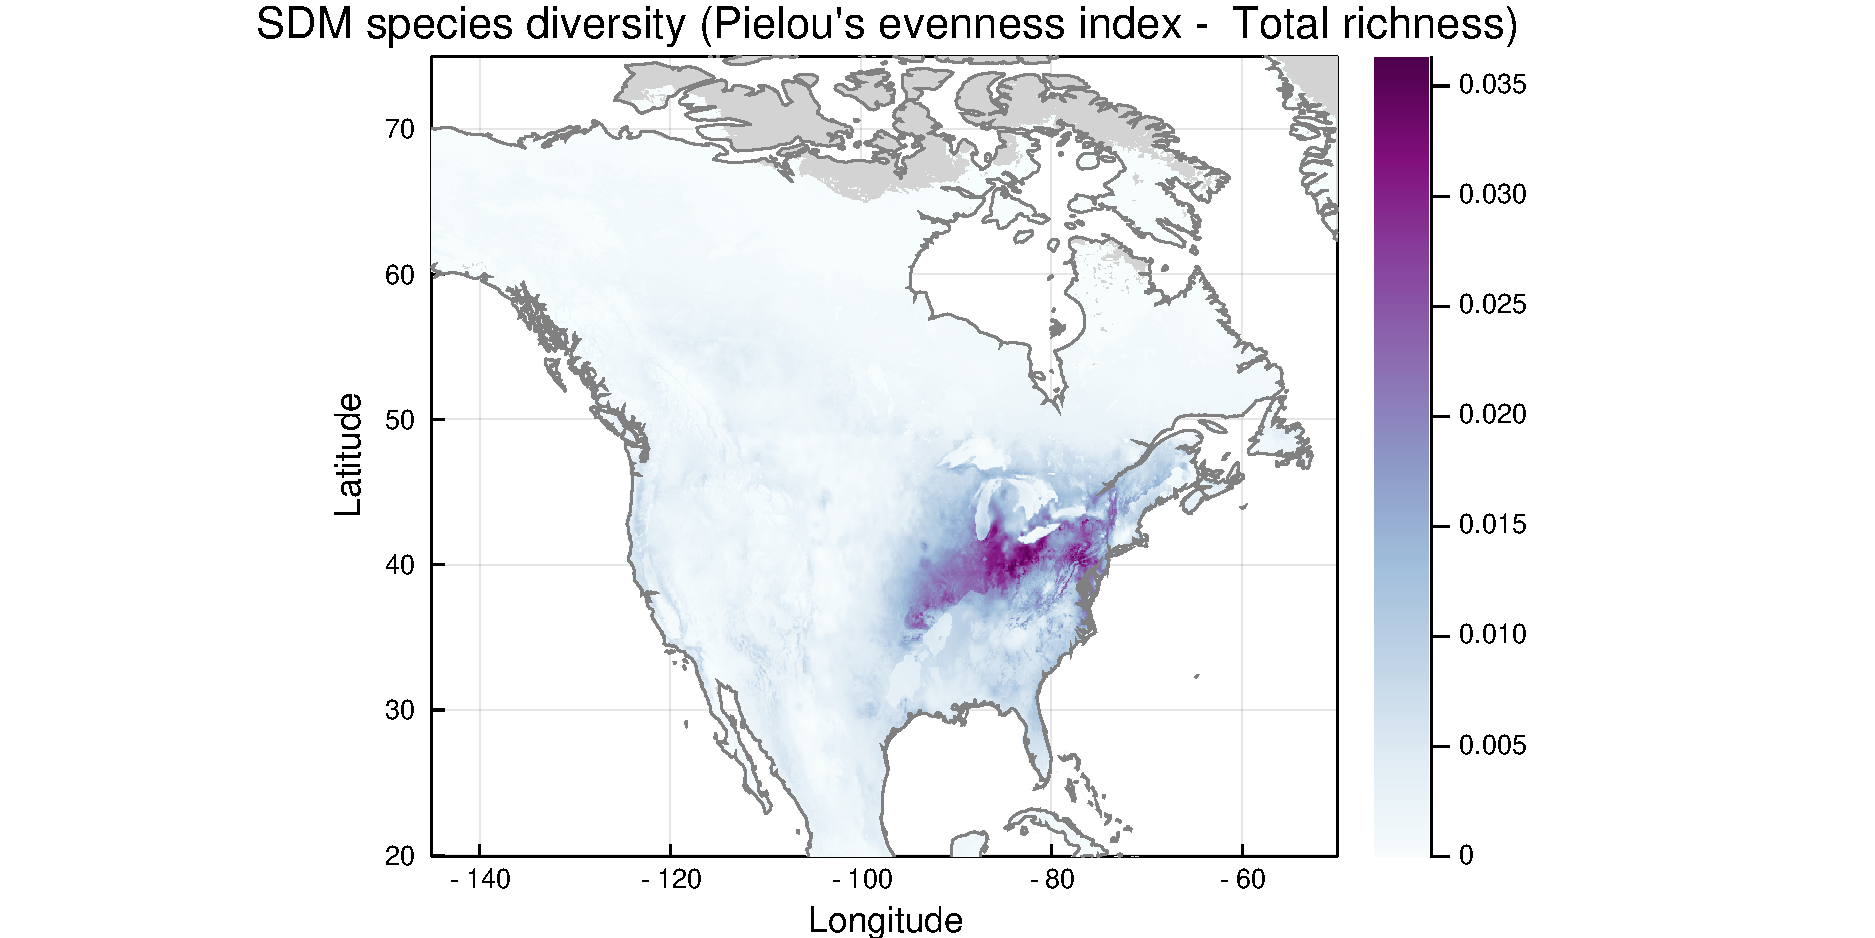
\includegraphics[scale=0.5]{../fig/sdm/sdm-diversity-pielou2.pdf}
  \end{figure}
\end{frame}

\begin{frame}
  \frametitle{SDM - Diversité spécifique}
  \begin{figure}
    \centering
    \hspace*{-2cm}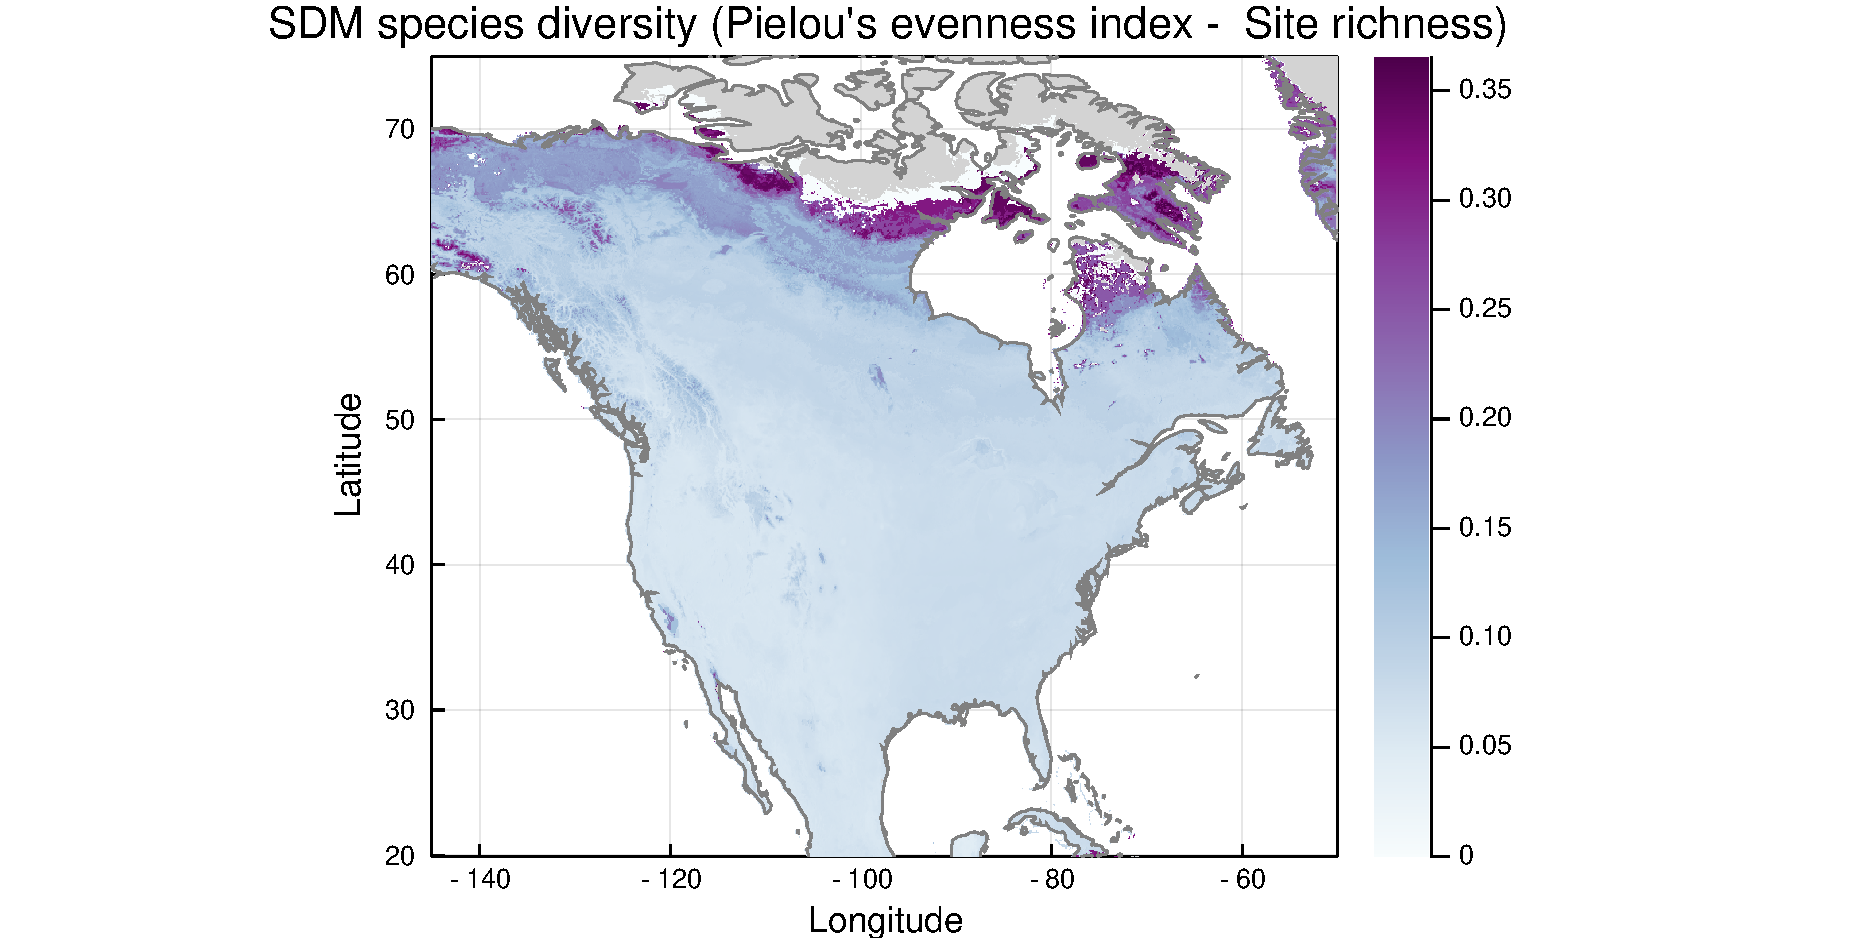
\includegraphics[scale=0.5]{../fig/sdm/sdm-diversity-pielou.pdf}
  \end{figure}
\end{frame}

\begin{frame}
  \frametitle{SDM - LCBD}
  \begin{figure}
    \centering
    \hspace*{-2cm}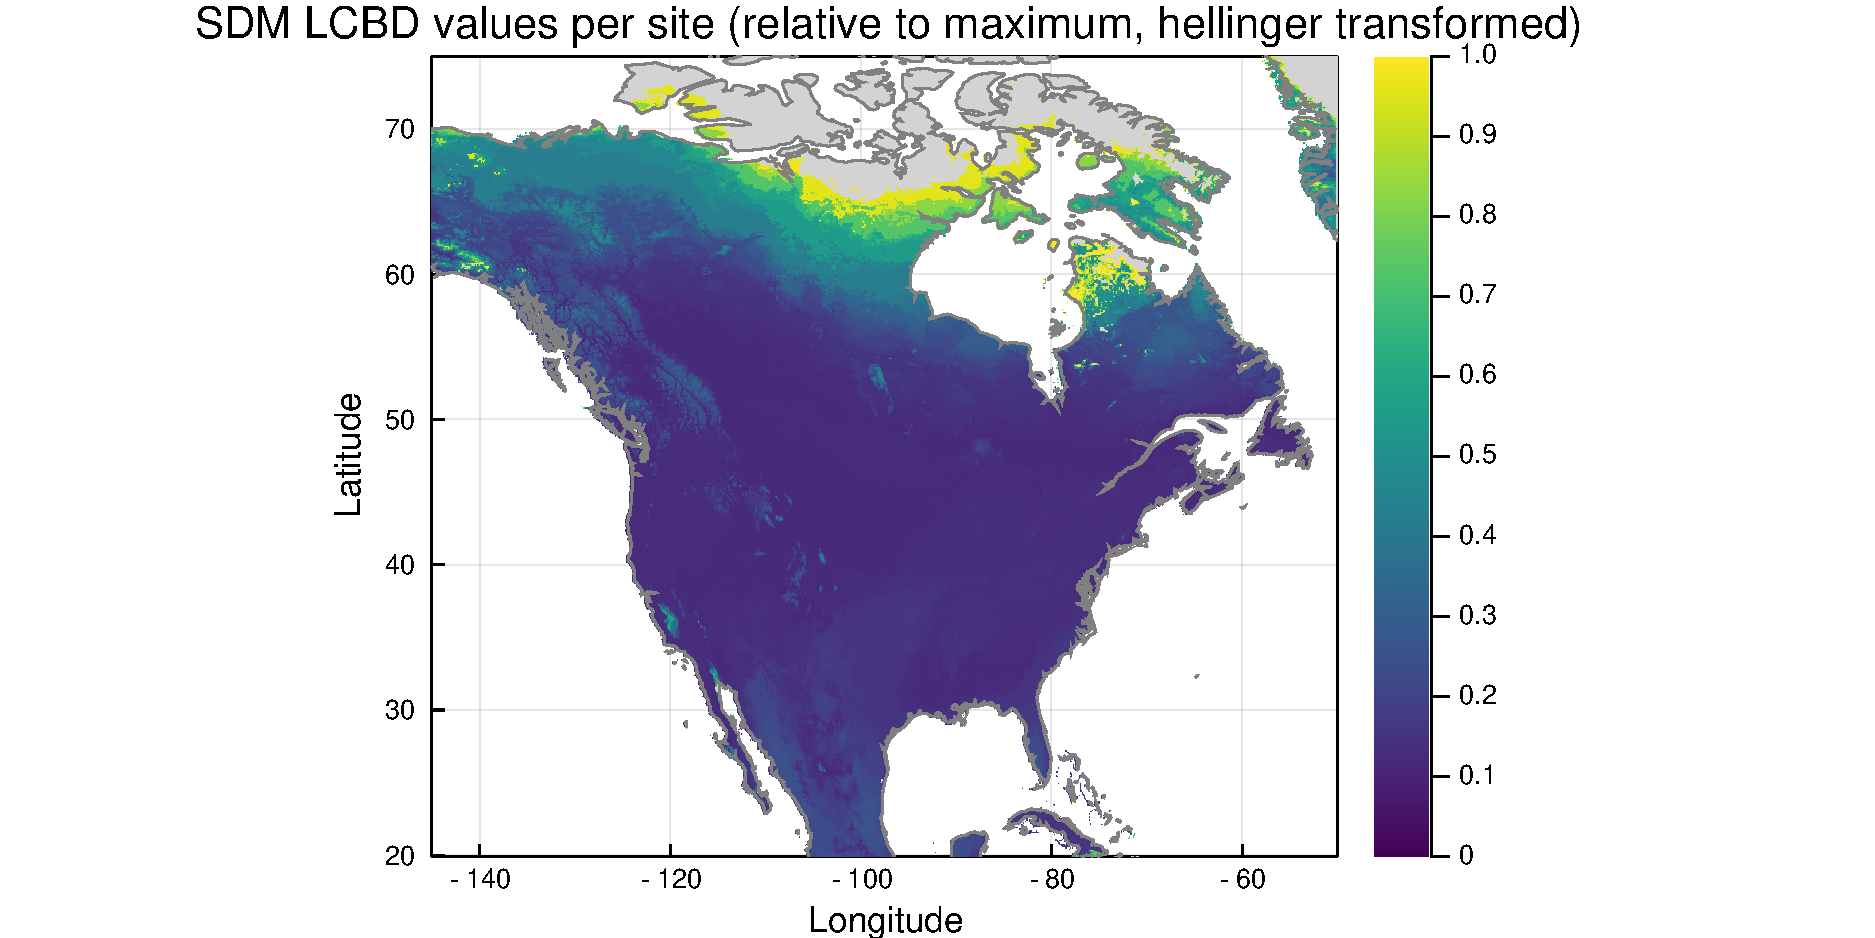
\includegraphics[scale=0.5]{../fig/sdm/sdm-lcbd-transf.pdf}
  \end{figure}
\end{frame}

\begin{frame}
  \frametitle{SDM - LCBD significatives}
  \begin{figure}
    \centering
    \hspace*{-2cm}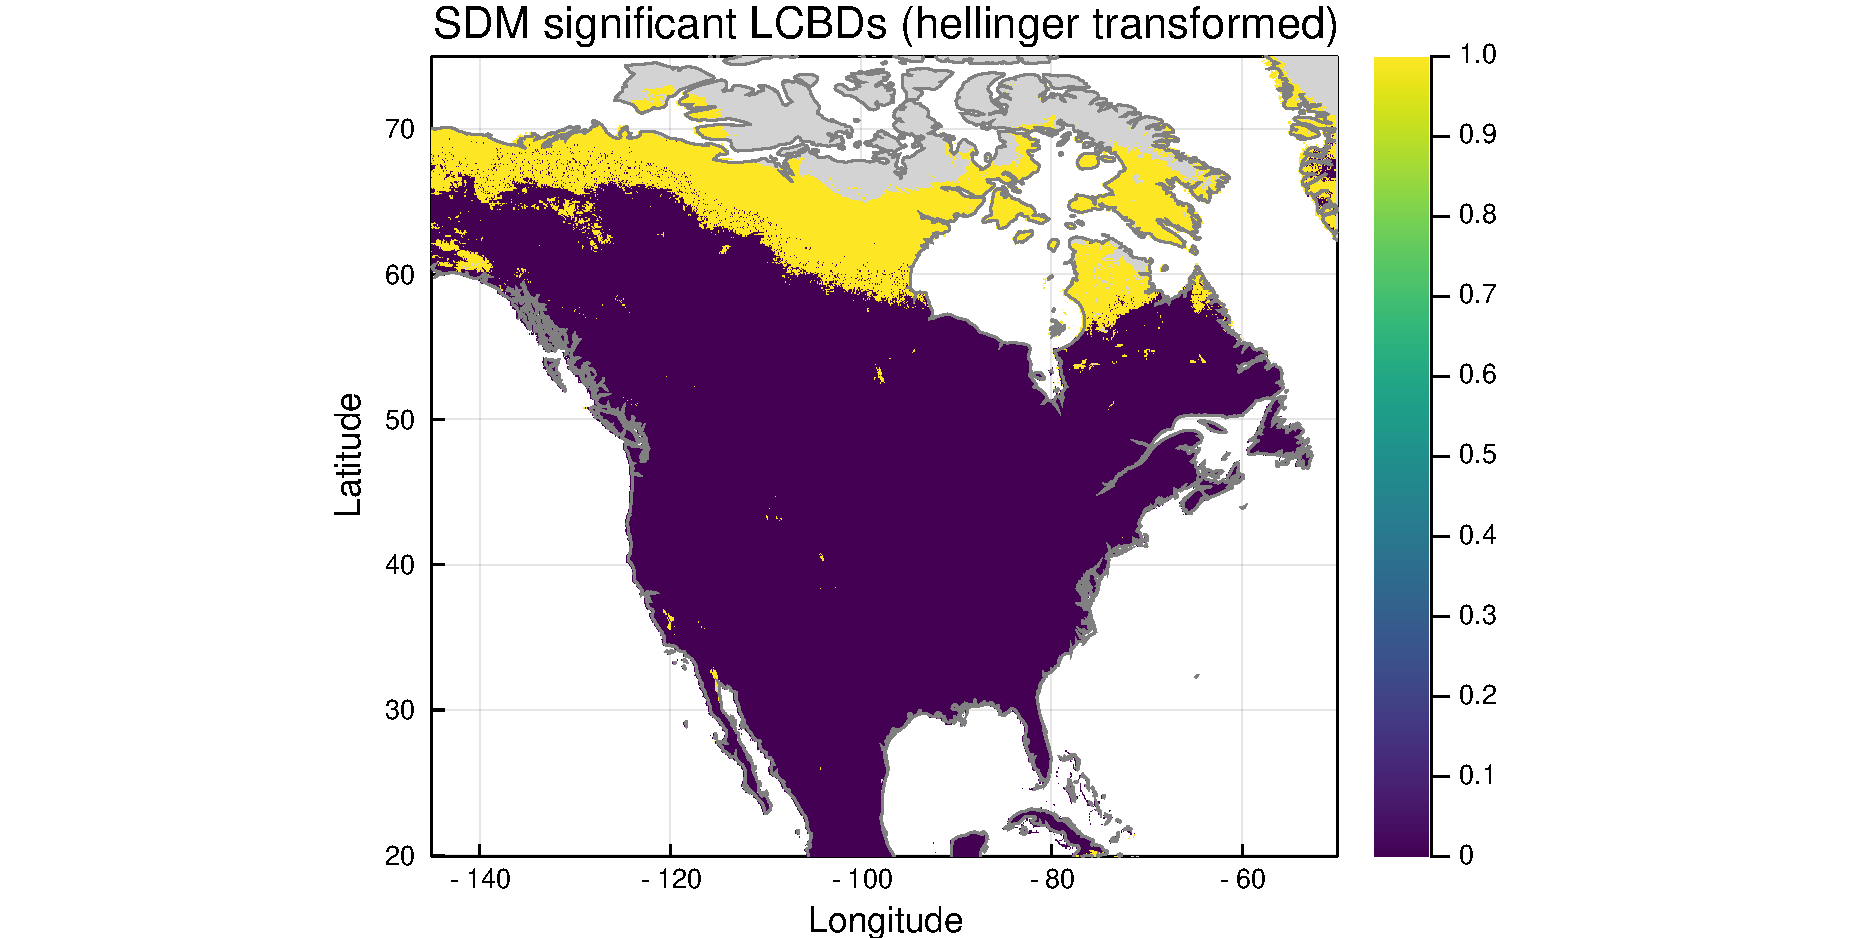
\includegraphics[scale=0.5]{../fig/sdm/sdm-lcbd-signif.pdf}
  \end{figure}
\end{frame}

\begin{frame}
  \frametitle{SDM - Relation LCBD-richesse}
  \begin{figure}
    \centering
    \hspace*{-2cm}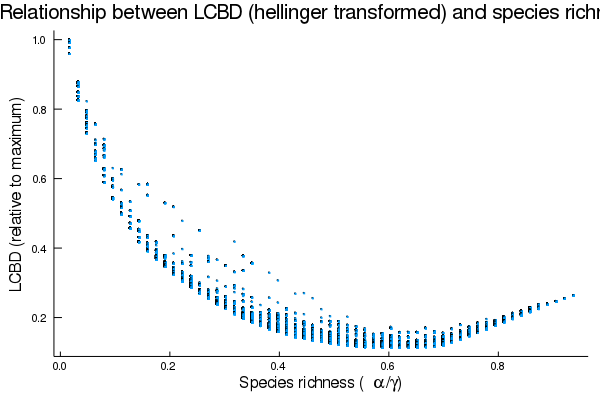
\includegraphics[scale=0.5]{../fig/sdm/sdm-relation-lcbd-richness-transf.png}
  \end{figure}
\end{frame}

\begin{frame}
  \frametitle{À venir}
  \begin{itemize}
    \item Échantillonnage Checklists par pixel
    \item Random Forests
    \item Prévisions changements climatiques
    \item Données d'interactions
  \end{itemize}
\end{frame}

\begin{frame}
  \frametitle{Autres points}
  \begin{itemize}
    \item Formation comité-conseil
    \item Travail BIO6077
  \end{itemize}
\end{frame}

\end{document}
